\subsection{Début de partie}

\subsubsection{Fenêtre initiale}
Au début de la partie, l'écran suivant s'affiche. Il est possible de créer ou charger une partie. Pour le chargement d'une partie, il faut taper le nom de la sauvegarde que l'on veut charger, et valider.

\begin{figure}[ht!]
\centering
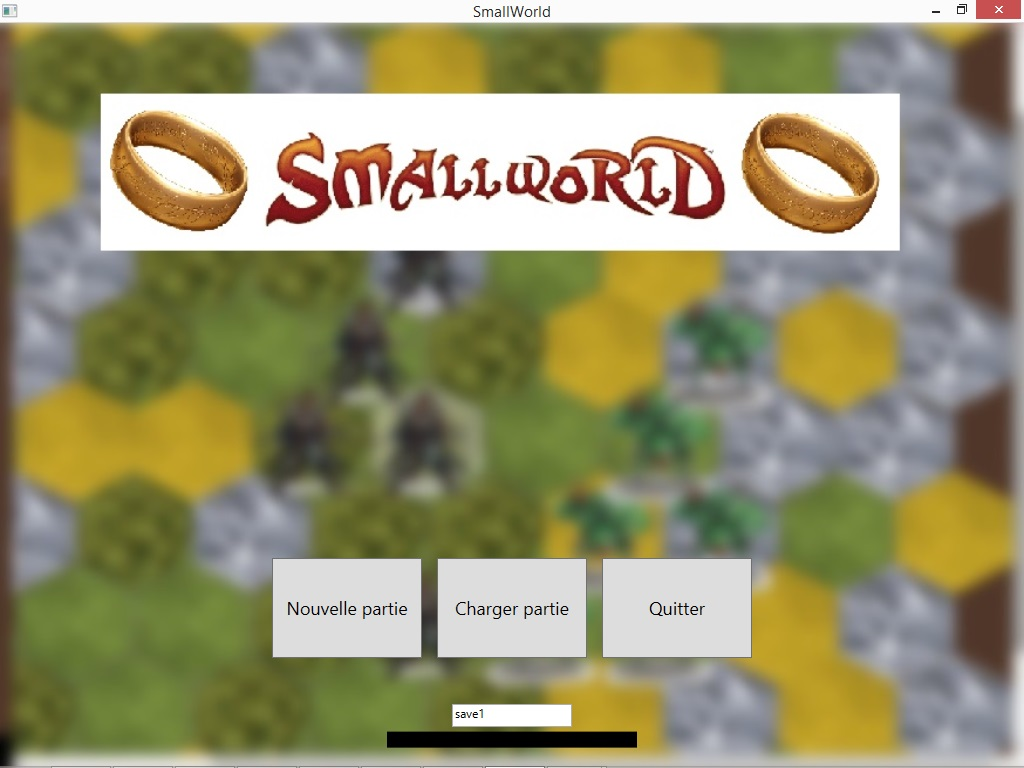
\includegraphics[scale=0.40]{img/init.jpg}
\caption{Fenêtre initiale}
\end{figure}

\subsubsection{Fenêtre de création de partie}
Puis l'écran suivant s'affiche. Le premier joueur doit choisir son type de créature et rentrer son nom de joueur. Puis il valide. Après, c'est autour du second joueur, qui fera de même. Après avoir validé, la partie est lancée.

\begin{figure}[ht!]
\centering
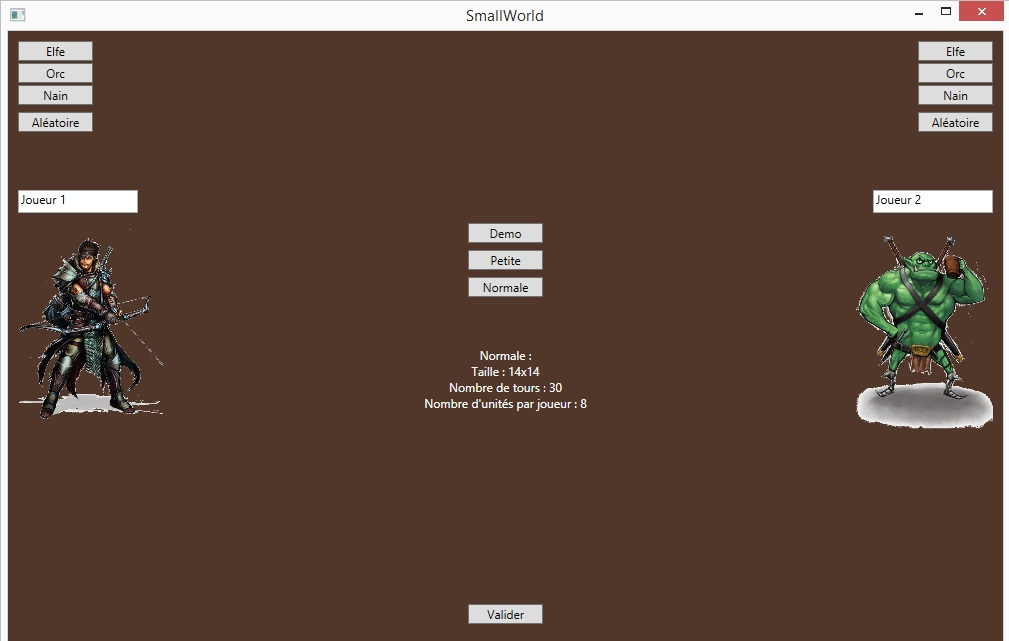
\includegraphics[scale=0.40]{img/crea.jpg}
\caption{Fenêtre de création de partie}
\end{figure}


\subsubsection{Fenêtre de jeu}
Au cours de la partie, c'est la fenêtre suivante qui s'affiche. On remarque en haut à gauche que c'est au joueur 1 "Jean-Pierre" de jouer. Le nombre d'anneaux des deux joueurs est affiché au milieu.

\begin{figure}[ht!]
\centering
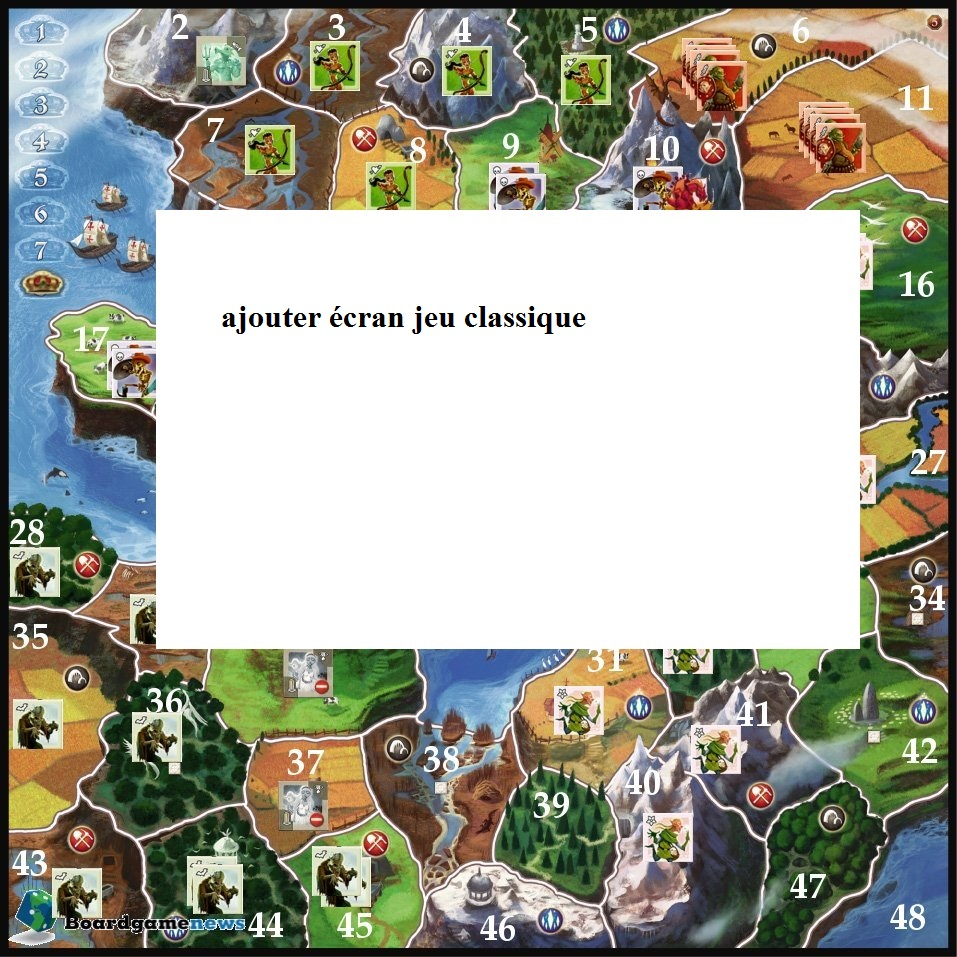
\includegraphics[scale=0.40]{img/jeu.jpg}
\caption{Fenêtre de jeu}
\end{figure}

\subsection{Déroulement d'un tour}

XOXO

\subsubsection{Généralités}

XOXO

\subsubsection{Actions du jeu}

XOXO

\subsection{Fin de partie}

Au bout d'un certain nombre de tours, la partie prend fin. 
\newline
L'enchantement de Saruman fait effet et le joueur contrôlant le plus d'anneaux de contrôle retrouve l'anneau unique. 
\newline
\newline
La partie est gagnée !
\newline
\newline
En cas de match nul, les deux joueurs reçoivent chacun une moitié de l'anneau unique, qui n'a plus grande valeur évidemment.